\section{Introduction}
\label{sec:intro}


In the realm of long-form text generation, a notable vulnerability of large language models (LLMs) is their propensity for hallucination, wherein the generated text contains factually inaccurate information.
By prepending the input prompt with relevant documents from trustworthy sources, retrieved-augmented generation (RAG)~\citep{lewis-etal-2021-rag,shi-etal-2024-replug} has been shown to be a simple yet effective approach that substantially mitigates the hallucination issue.
To further enhance the factual accuracy of model output, various iterative prompting methods have been proposed that build upon RAG. For instance, FLARE~\citep{jiang-etal-2023-active} generates responses sentence by sentence, and if a newly generated sentence contains low-probability tokens, it retrieves a new set of documents and re-runs RAG to regenerate the sentence. Alternatively, Self-RAG~\citep{asai2024selfrag} employs a self-critic component to verify the correctness of each partial generation and repeatedly queries a retrieval system to update the background knowledge, thereby producing more accurate and faithful responses.
While these systems demonstrate significant empirical improvement, they are restricted in the traditional RAG design. Context-relevant knowledge through retrieval is the only online feedback to the model, incorporated as part of the input string. 



In this work, we propose \model (\textbf{E}xplicit \textbf{W}orking m\textbf{E}mory), an iterative framework that aims to provide more factual responses for knowledge-intensive long-form generation, with the help of an auxiliary fact-checking module. \model augments an existing language model with an explicit working memory, which keeps track of the knowledge that is most relevant and useful at the current generation timestep. The memory is initially filled with the latent representation of some retrieved passages relevant to the input prompt. During the generation process, \model actively monitors the newly generated partial response and pauses occasionally to refresh the memory with knowledge from retrieval and to 
check the output statement. If the statement is factually incorrect, it then refreshes the memory with the fact-checking feedback. With the updated memory, \model first removes the incorrect statement and backtracks to the previous timestep, and then continues the generation process from there. 

\begin{figure}
    \centering
    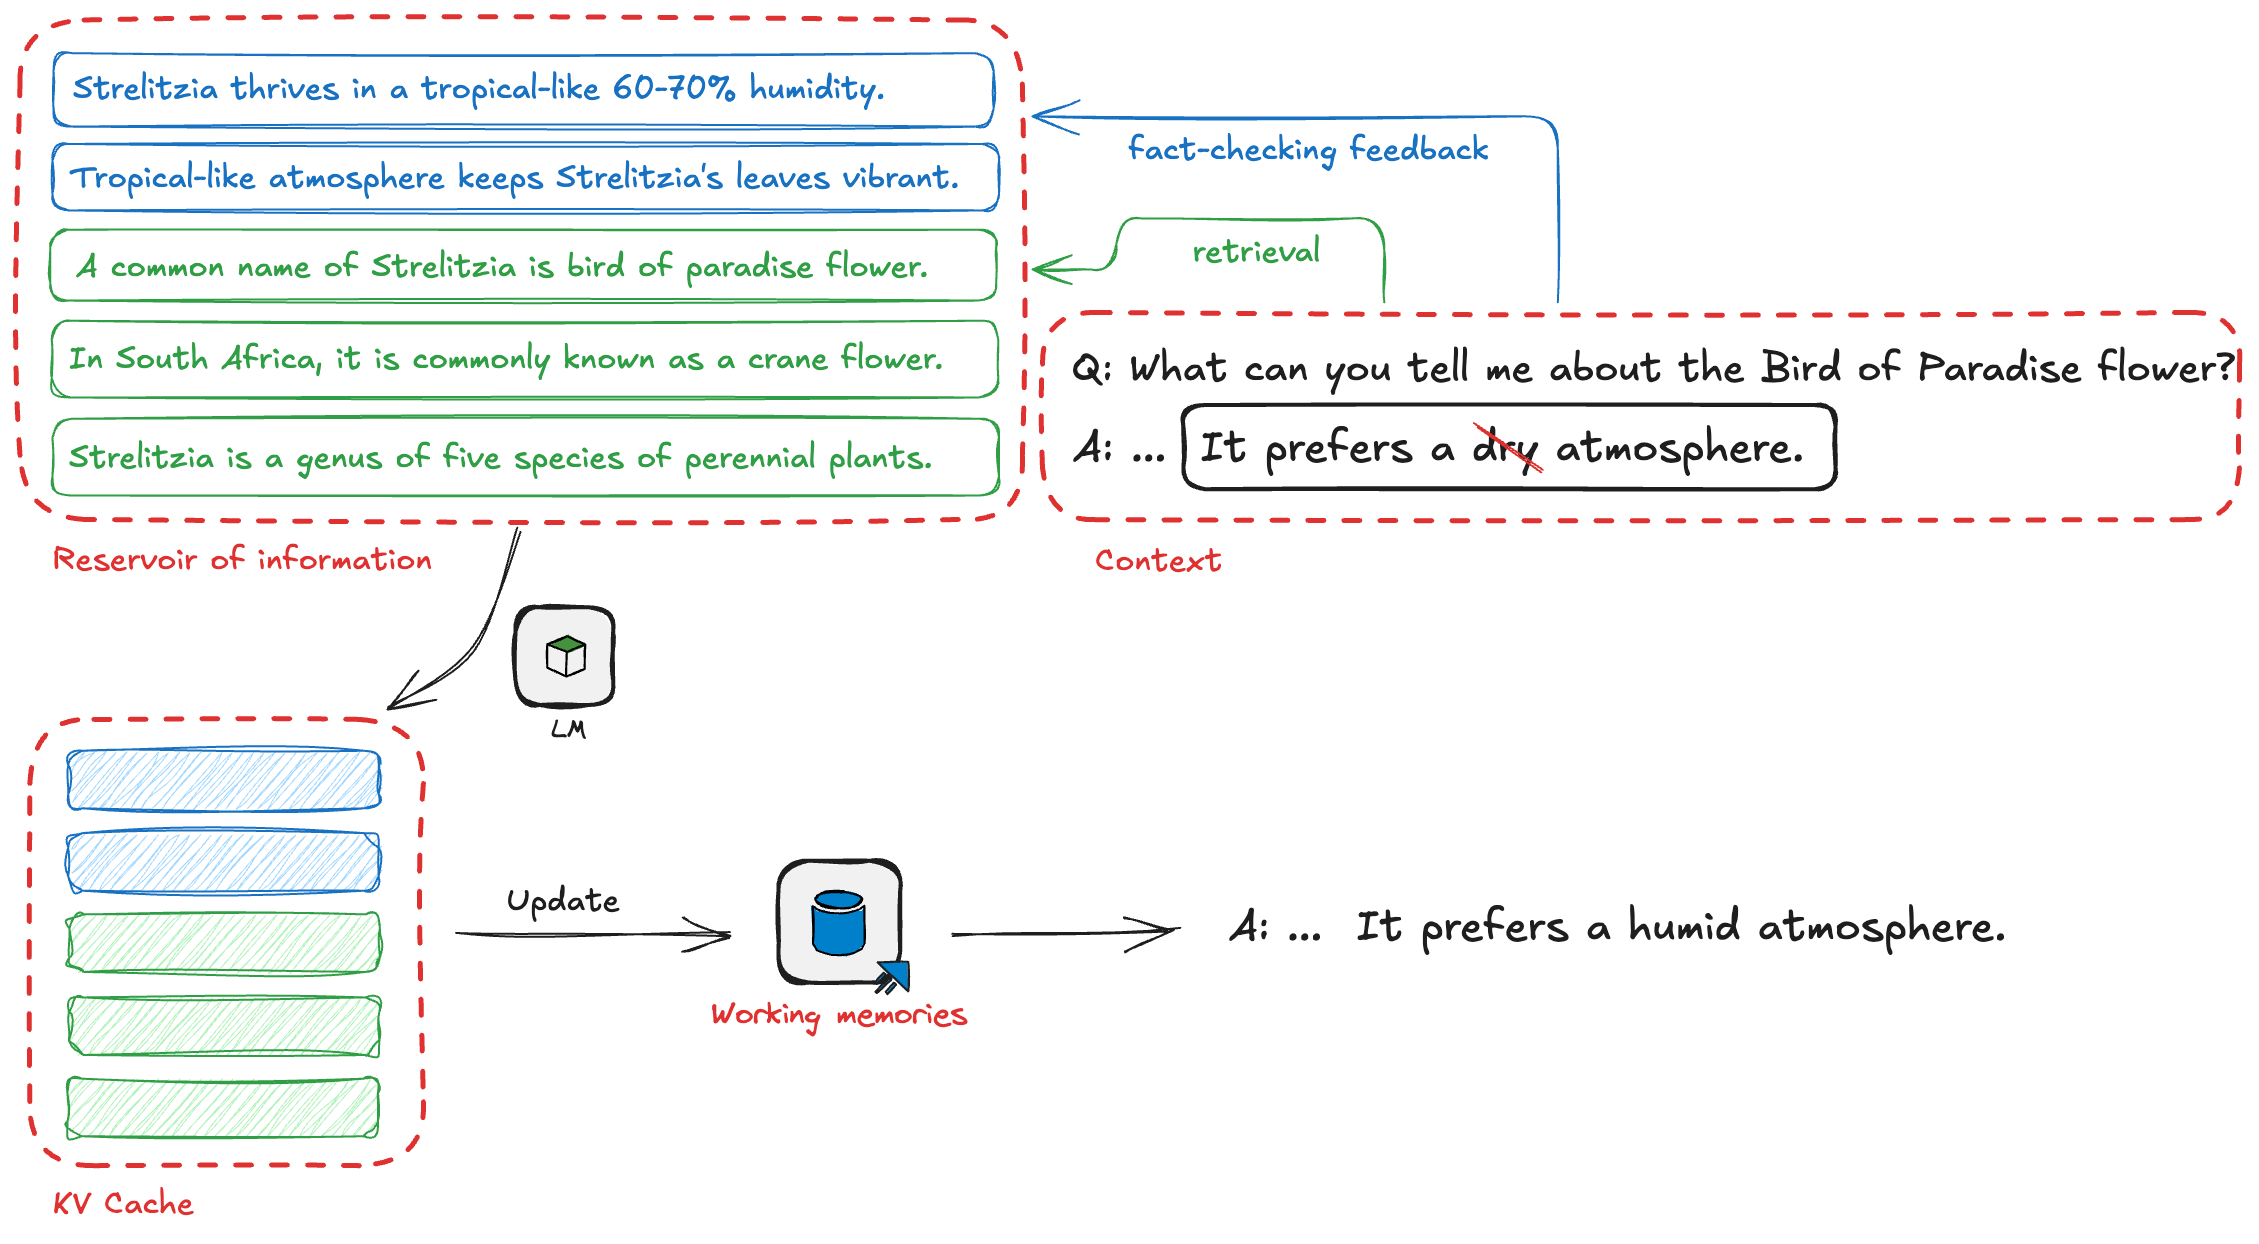
\includegraphics[width=\textwidth]{figures/intro_fig.png}
    \caption{Example pipeline illustrating how \model pauses, receives feedback from retrievers and fact-checkers, and then re-generate to correct factual errors in its outputs. \model handles knowledge from fact-checkers and retrievers separately as they tend to provide information with distinct properties. Retrieval offers more general background information, while fact-checkers focus more on specific details, targeting particular aspects of the output text.}
    \label{fig:intro}
\end{figure}



We assume that the main text generation model used here is a Transformer-based large language model, such as Llama~\citep{dubey2024llama3herdmodels}. Similar to the standard RAG setting, given an input prompt, we first retrieve $k$ relevant text chunks of the same number of tokens, as the background knowledge. Unlike RAG, which directly prepends the input prompt with these $k$ chunks, we apply the language model to them separately and store the KV cache of each chunk in a memory of $k$ units. When predicting the next token, the language model effectively attends the current token to all $k$ chunks in parallel, using their KV caches stored in the memory, and have the average as the attention value. 
When \model pauses the generation and checks the newly generated, partial response, it has the opportunity to update the memory in multiple ways to guide the language model. For instance, if some claims in the new sentence are not supported, this feedback along with additional supporting documents can be used as a new unit appended to the existing memory. In addition, if the knowledge from an initial retrieved passage is no longer relevant, its corresponding memory unit can be removed or updated with embeddings of a new passage retrieved using the generated partial response as query. 

\model can be seen as a more general framework that subsumes many existing approaches. For example, if there is no stopping in generation and if the memory contains only one unit (i.e., $k$=1), then \model degenerates to the simple vanilla RAG. If \model pauses at the end of generation of every sentence and checks whether the new sentence contains any token with low probability as a proxy of factuality measure, then this particular instantiation, with one memory unit, is effectively FLARE. Notice that in a typical, more general configuration of \model, the memory module consists of multiple units. When the memory is refreshed, not all the units need to be updated. If some knowledge is still required, their original raw data (e.g., passages) will not be reprocessed to create the embeddings, saving some redundant computational cost at inference time.
While conceptually simple, the working memory design in \model provides a more flexible and yet efficient way to incorporate various of types of external online information, as different forms of feedback are encoded in parallel and stored in memory units (e.g., see Figure~\ref{fig:intro}).
We notice that the design of leveraging working memory is also very related to some recently proposed methods for long-content models (e.g., Memory$^3$~\citep{yang2024text}). If our memory is used only for encoding the knowledge from the passages in our corpus, then this can be viewed as the whole corpus is used as the context, along with the prompt, as the input to the model. The key differences are that \model does not pre-encode every passage (although the KV caches of some frequently retrieved passages can certainly be precomputed in advance) and its memory can be dynamically updated as the generation progresses.

We demonstrate empirically that \model generates more factual responses without sacrificing the relevance to the input questions, using four fact-seeking long-form generation datasets. In general, with the feedback from online fact-checking and targeted retrieval, \model increases \vs~\citep{song-etal-2024-veriscore}, the factuality metric we use, by 2 to 10 points absolute and has a similar helpfulness in terms of instruction following compared to the base model Llama-3.1$_\text{70B}$.
